\documentclass[oneside,final]{hcmut-report}
\usepackage{codespace}
\usepackage{gensymb,textcomp}
\usepackage{array,longtable,multicol,multirow,siunitx,tabularx}
\usepackage{enumitem}
\usepackage{caption,float}
\usepackage[export]{adjustbox}
\usepackage[nameinlink]{cleveref}
\usepackage{fancyhdr}
\usepackage{lastpage}
\usepackage{xcolor}

\pagestyle{fancy}
\fancyhf{}
\fancyhead[L]{%
    \begin{tabular}[b]{@{}l@{}}
        Ho Chi Minh City University of Technology \\
        Faculty of Computer Science and Engineering
    \end{tabular}%
}
\fancyhead[R]{%
    \raisebox{-0.15\height}{
\includegraphics[height=1.0cm]{graphics/hcmut.png}}%
}
\fancyfoot[C]{\thepage}
\renewcommand{\headrulewidth}{0.4pt}
\renewcommand{\footrulewidth}{0pt}

% ==================== THÔNG TIN BÁO CÁO ====================
\coursename{COMPUTER NETWORK REPORT}
\reporttype{LAB 7: WIRESHARK 802.11 WIFI}
\title{Homework 2b}
\advisor{ &}
\stuname{ &}
\reportplace{HO CHI MINH CITY}
\reporttime{NOVEMBER 2026}

\begin{document}

% Trang bìa theo mẫu hcmut-report
\coverpage

% ==================== MỤC LỤC ====================
\newpage
\tableofcontents
\newpage

% ==================== PHẦN 1: BEACON FRAMES ====================
\section{Beacon Frames}

\subsection{Question 1}
\textbf{Question:} What are the SSIDs of the two access points that are issuing most of the beacon frames in this trace?

\textbf{Answer:}
By filtering for 802.11 Beacon frames using the Wireshark display filter \texttt{wlan.fc.type\_subtype == 0x08}, we analyze all beacon frames present in the trace. Out of 754 total beacon frames:
\begin{itemize}[noitemsep]
    \item \textbf{Access Point 1:} SSID \textbf{\texttt{"30 Munroe St"}} (BSSID: \texttt{00:16:b6:f7:1d:51}) accounts for \textbf{718 beacon frames} (over 95\% of all beacons).
    \item \textbf{Access Point 2:} SSID \textbf{\texttt{"linksys12"}} (BSSID: \texttt{00:06:25:67:22:94}) accounts for \textbf{25 beacon frames}.
\end{itemize}
Therefore, the two access points issuing most of the beacon frames in this trace are \textbf{30 Munroe St} and \textbf{linksys12}.

\begin{figure}[H]
    \centering
    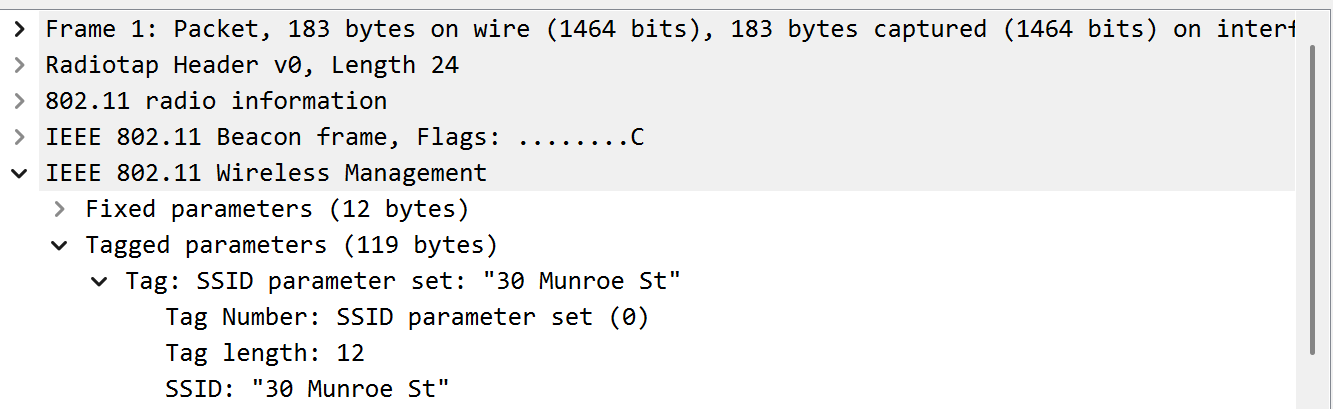
\includegraphics[width=0.95\linewidth]{graphics/fig1(1).png}
    \caption{Beacon Frame 1 showing SSID parameter set: \texttt{"30 Munroe St"}.}
\end{figure}

\begin{figure}[H]
    \centering
    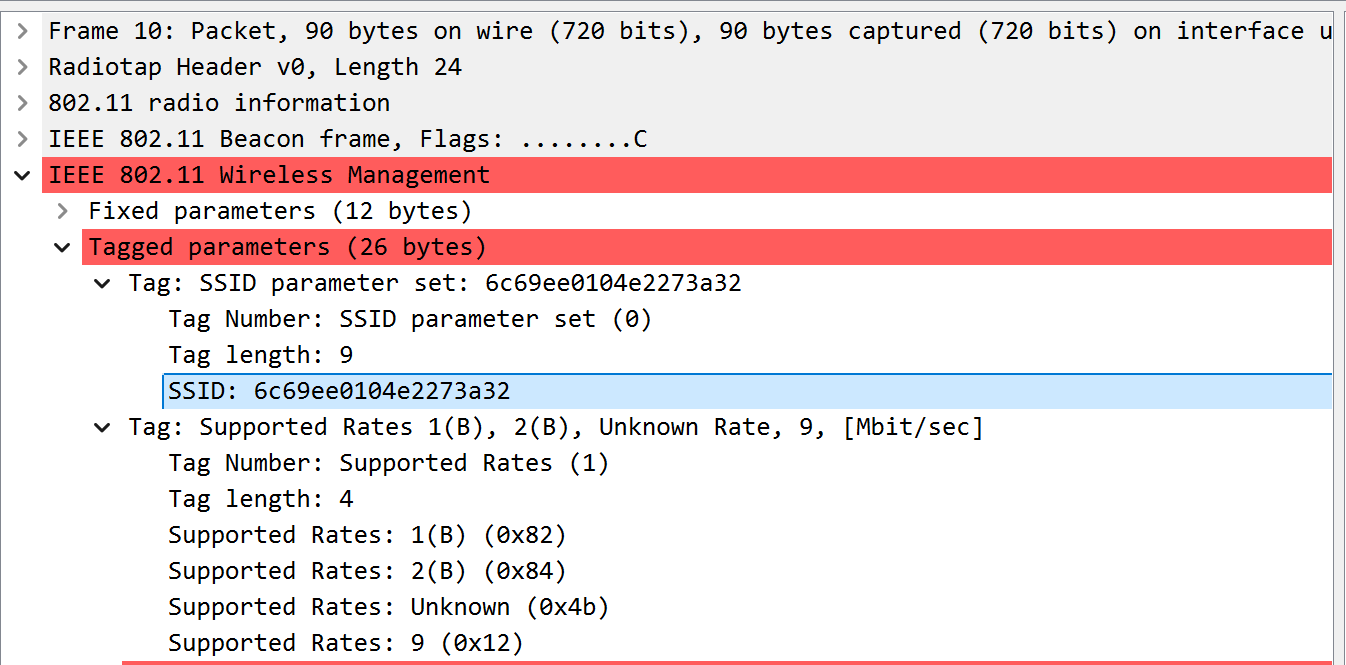
\includegraphics[width=0.95\linewidth]{graphics/fig1(2).png}
    \caption{Beacon Frame 10 showing SSID parameter set for the second access point (\textit{linksys}).}
\end{figure}

\subsection{Question 2}
\textbf{Question:} What are the intervals of time between the transmissions of the beacon frames from the \textit{linksys\_ses\_24086} access point? From the \textit{30 Munroe St.} access point? (Hint: this interval of time is contained in the beacon frame itself).

\textbf{Answer:}
The beacon interval is advertised inside the fixed parameters field of the IEEE 802.11 management frame (\texttt{wlan.fixed.beacon\_interval}). In the 802.11 standard, 1 Time Unit (TU) equals $1024\,\mu\text{s} = 0.001024\,\text{s}$:
\begin{itemize}[noitemsep]
    \item \textbf{30 Munroe St} (Frame 1): \textbf{0.102400 seconds} (100 Time Units).
    \item \textbf{linksys\_ses\_24086} (Frame 1774): \textbf{0.102400 seconds} (100 Time Units).
\end{itemize}
Both access points specify a target beacon transmission interval of \textbf{100 TU (102.4 ms)}, which is the standard default for 802.11 Wi-Fi networks.

\begin{figure}[H]
    \centering
    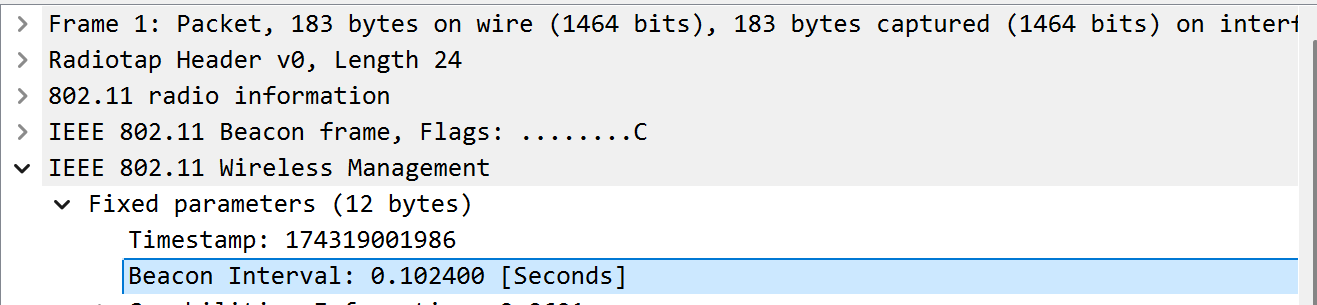
\includegraphics[width=0.95\linewidth]{graphics/fig2(1).png}
    \caption{Fixed parameters of Beacon Frame 1 showing \textit{Beacon Interval: 0.102400 [Seconds] (100 TU)}.}
\end{figure}

\subsection{Question 3}
\textbf{Question:} What (in hexadecimal notation) is the source MAC address on the beacon frame from 30 Munroe St?

\textbf{Answer:}
Examining Frame 1 (a beacon frame transmitted by \textit{30 Munroe St}), the Transmitter/Source MAC address is specified in the \textbf{Address 2} field of the IEEE 802.11 MAC header:
\begin{itemize}[noitemsep]
    \item \textbf{Source MAC Address (Address 2 / SA):} \texttt{00:16:b6:f7:1d:51} (\texttt{CiscoLinksys\_f7:1d:51}).
\end{itemize}

\subsection{Question 4}
\textbf{Question:} What (in hexadecimal notation) is the destination MAC address on the beacon frame from 30 Munroe St??

\textbf{Answer:}
In Frame 1, the Destination/Receiver MAC address is located in the \textbf{Address 1} field of the IEEE 802.11 header:
\begin{itemize}[noitemsep]
    \item \textbf{Destination MAC Address (Address 1 / DA):} \texttt{ff:ff:ff:ff:ff:ff} (Broadcast).
\end{itemize}
Because beacon frames announce network presence to all nearby wireless stations in range, they are broadcasted to the universal broadcast address.

\subsection{Question 5}
\textbf{Question:} What (in hexadecimal notation) is the MAC BSS id on the beacon frame from 30 Munroe St?

\textbf{Answer:}
In IEEE 802.11 infrastructure mode, the BSSID is the MAC address of the AP's wireless interface, contained in the \textbf{Address 3} field of the beacon frame:
\begin{itemize}[noitemsep]
    \item \textbf{MAC BSS ID (Address 3 / BSSID):} \texttt{00:16:b6:f7:1d:51} (\texttt{CiscoLinksys\_f7:1d:51}).
\end{itemize}

\begin{figure}[H]
    \centering
    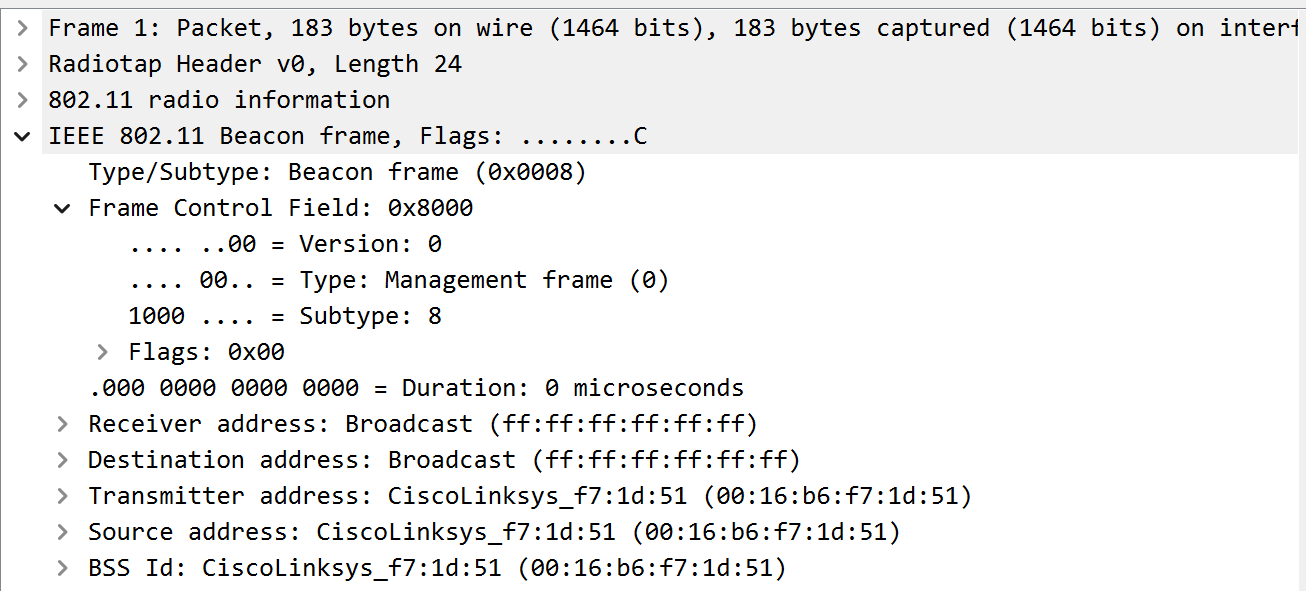
\includegraphics[width=0.95\linewidth]{graphics/fig3_4_5(1).png}
    \caption{IEEE 802.11 Header of Frame 1 displaying Receiver/Destination (\texttt{ff:ff:ff:ff:ff:ff}), Transmitter/Source (\texttt{00:16:b6:f7:1d:51}), and BSS Id (\texttt{00:16:b6:f7:1d:51}).}
\end{figure}

\subsection{Question 6}
\textbf{Question:} The beacon frames from the 30 Munroe St access point advertise that the access point can support four data rates and eight additional “extended supported rates.” What are these rates?

\textbf{Answer:}
Looking into the \textit{Tagged parameters} section of Frame 1:
\begin{itemize}[noitemsep]
    \item \textbf{Supported Rates (Tag 1, 4 rates):} \textbf{1.0, 2.0, 5.5, 11.0 Mbit/sec} (standard 802.11b DSSS basic rates).
    \item \textbf{Extended Supported Rates (Tag 50, 8 rates):} \textbf{6.0, 9.0, 12.0, 18.0, 24.0, 36.0, 48.0, 54.0 Mbit/sec} (standard 802.11g OFDM rates).
\end{itemize}

\begin{figure}[H]
    \centering
    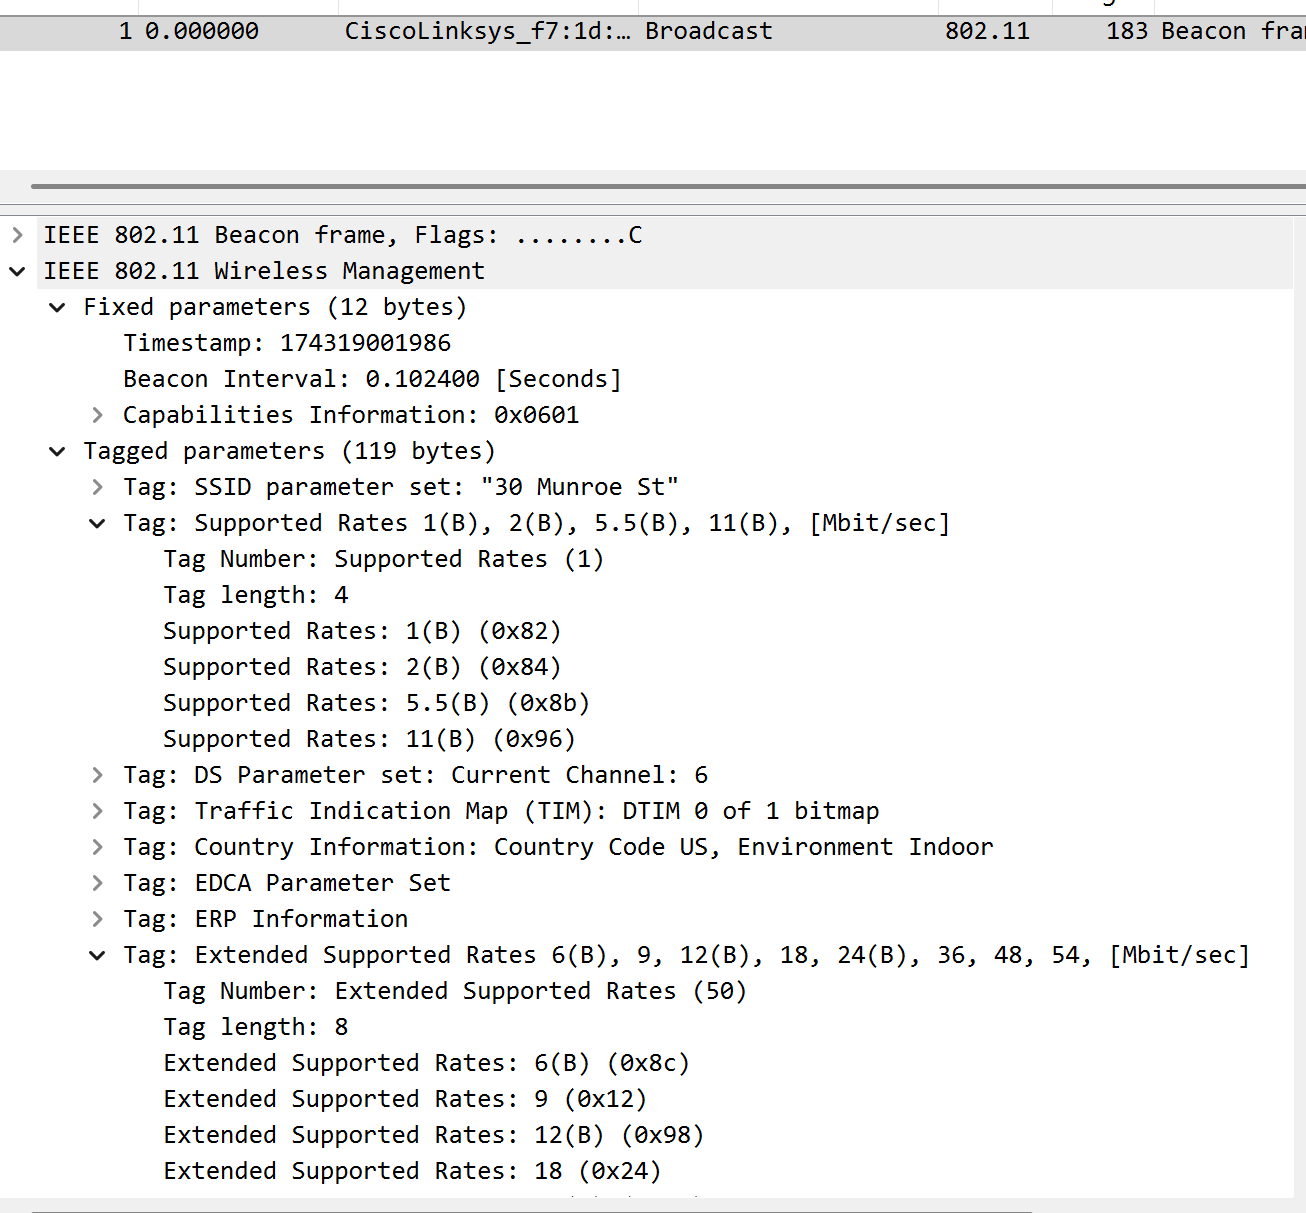
\includegraphics[width=0.95\linewidth]{graphics/fig6(1).png}
    \caption{Supported Rates (1, 2, 5.5, 11 Mbit/s) and Extended Supported Rates (6, 9, 12, 18, 24, 36, 48, 54 Mbit/s) in Frame 1.}
\end{figure}

% ==================== PHẦN 2: DATA TRANSFER ====================
\newpage
\section{Data Transfer}

\subsection{Question 7}
\textbf{Question:} Find the 802.11 frame containing the SYN TCP segment for this first TCP session (that downloads alice.txt). What are three MAC address fields in the 802.11 frame? Which MAC address in this frame corresponds to the wireless host (give the hexadecimal representation of the MAC address for the host)? To the access point? To the first-hop router? What is the IP address of the wireless host sending this TCP segment? What is the destination IP address? Does this destination IP address correspond to the host, access point, first-hop router, or some other network-attached device? Explain.

\textbf{Answer:}
Using the filter \texttt{tcp.flags.syn == 1 \&\& tcp.flags.ack == 0}, we locate \textbf{Frame 474} ($t = 24.811093\,\text{s}$).

\begin{enumerate}[noitemsep,label=\arabic*.]
    \item \textbf{Three MAC address fields in Frame 474:}
    \begin{itemize}[noitemsep]
        \item \textbf{Address 1 (Receiver Address - RA):} \texttt{00:16:b6:f7:1d:51} (\texttt{CiscoLinksys\_f7:1d:51}) $\rightarrow$ Corresponds to the \textbf{Access Point (AP)}.
        \item \textbf{Address 2 (Transmitter / Source Address - SA):} \texttt{00:13:02:d1:b6:4f} (\texttt{Intel\_d1:b6:4f}) $\rightarrow$ Corresponds to the \textbf{Wireless Host}.
        \item \textbf{Address 3 (Destination Address - DA):} \texttt{00:16:b6:f4:eb:a8} (\texttt{CiscoLinksys\_f4:eb:a8}) $\rightarrow$ Corresponds to the \textbf{First-hop router} (LAN/gateway interface).
    \end{itemize}
    \item \textbf{Wireless Host IP Address:} \texttt{192.168.1.109}.
    \item \textbf{Destination IP Address:} \texttt{128.119.245.12} (\texttt{gaia.cs.umass.edu}).
    \item \textbf{Explanation:} The destination IP address does \textbf{not} correspond to the host, the access point, or the first-hop router; it corresponds to an external remote web server hosting \texttt{alice.txt}. The wireless host addresses the link-layer frame to the AP (Address 1) to be forwarded to the first-hop router (Address 3), which decapsulates the link-layer header and routes the IP datagram across the wide-area Internet to the destination server.
\end{enumerate}

\begin{figure}[H]
    \centering
    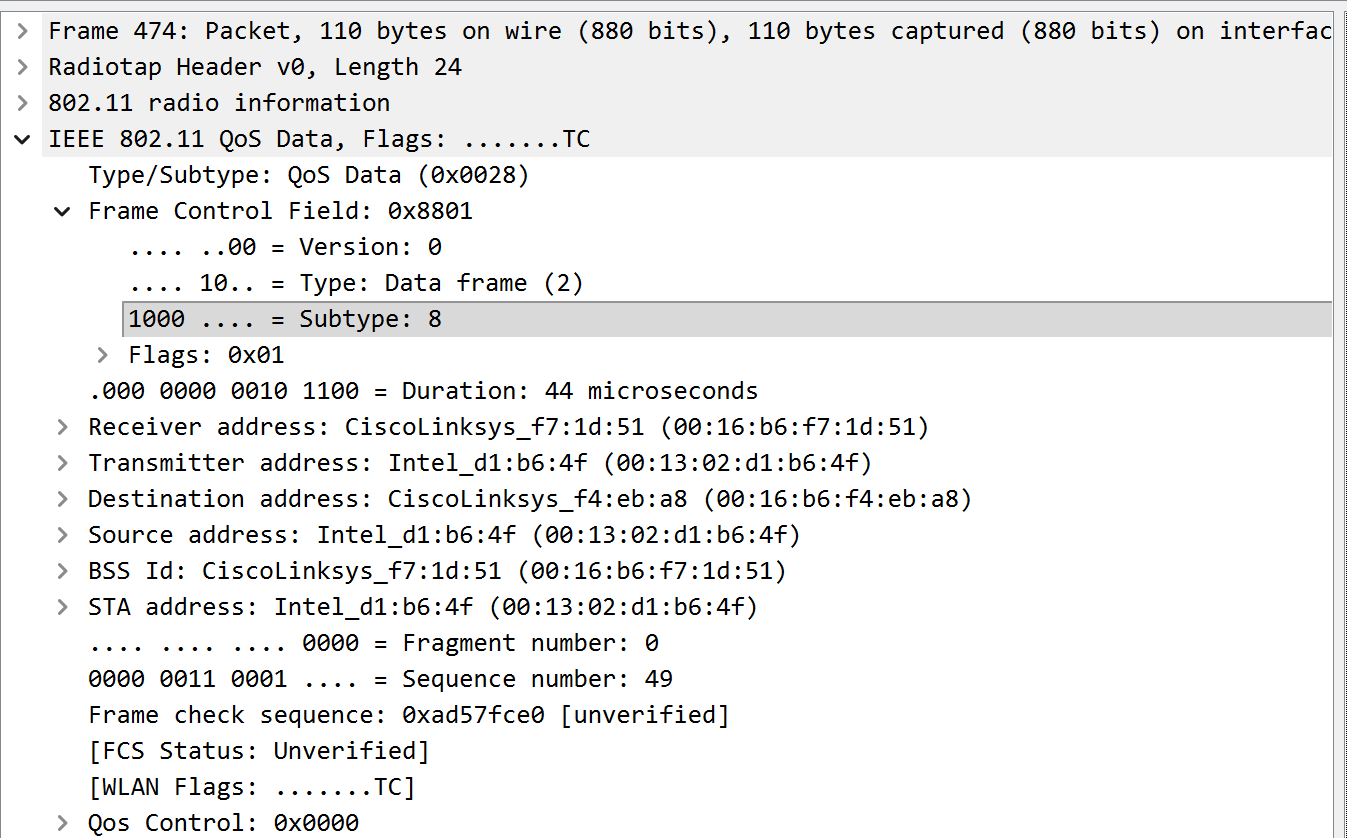
\includegraphics[width=0.95\linewidth]{graphics/fig7(1).png}
    \caption{Frame 474: 802.11 QoS Data header displaying Receiver (\texttt{00:16:b6:f7:1d:51}), Transmitter/Source (\texttt{00:13:02:d1:b6:4f}), and Destination router (\texttt{00:16:b6:f4:eb:a8}).}
\end{figure}

\begin{figure}[H]
    \centering
    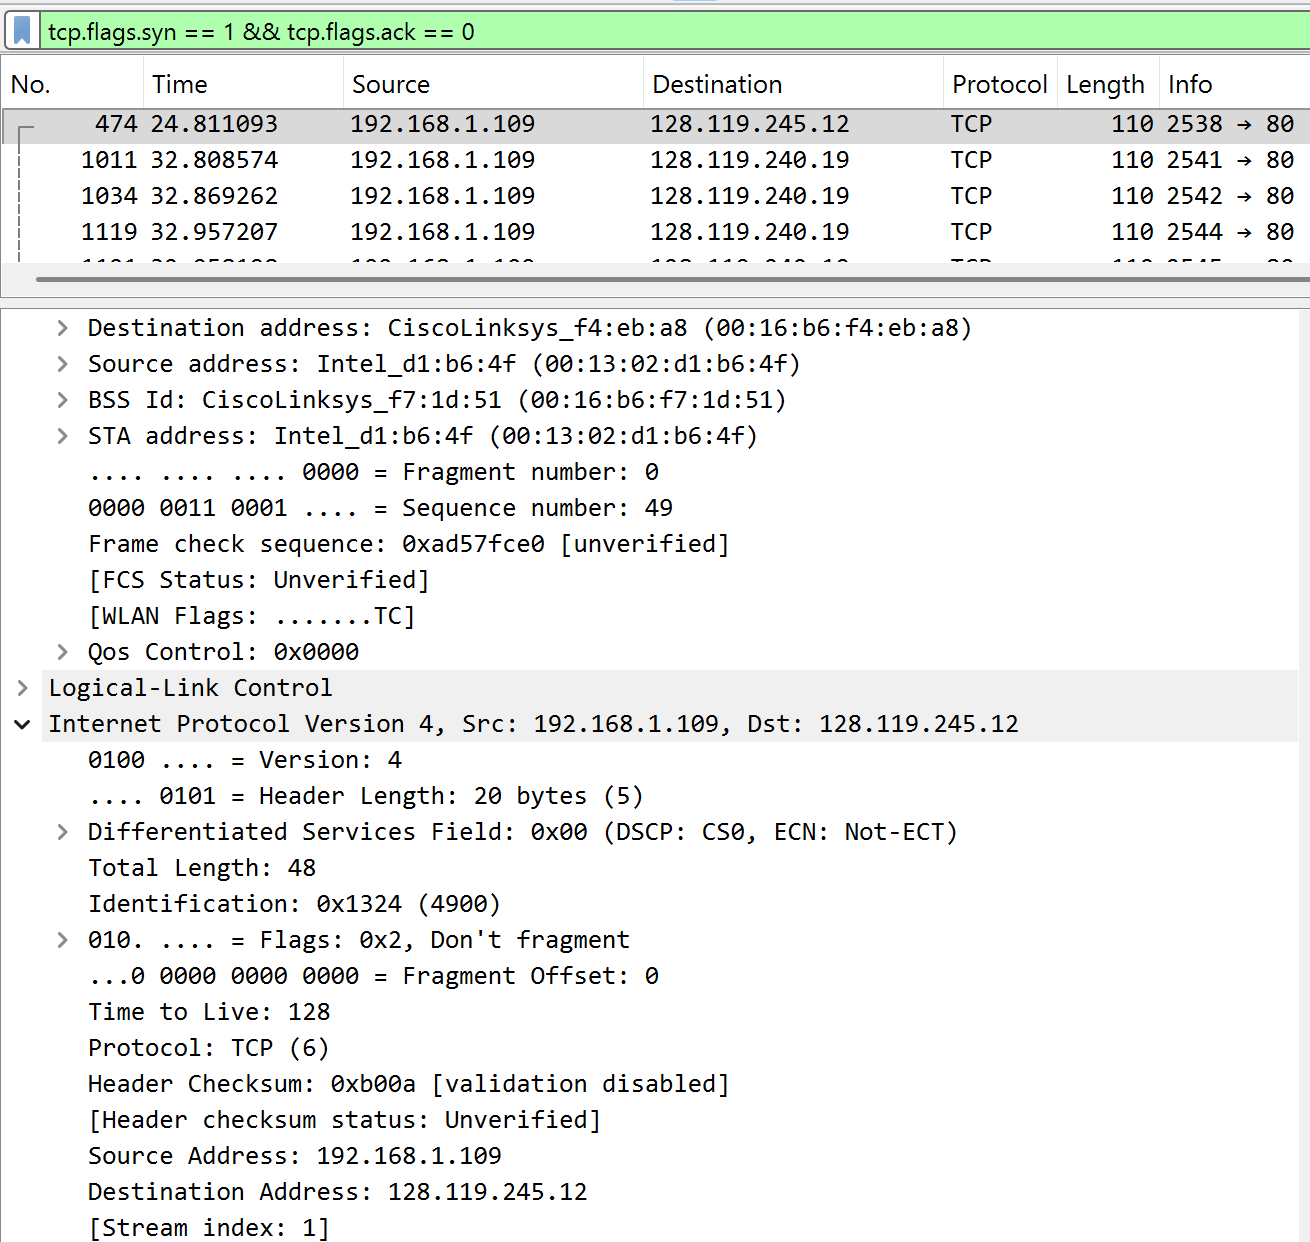
\includegraphics[width=0.95\linewidth]{graphics/fig7(2).png}
    \caption{Frame 474: Filter and IPv4 layer showing Source IP \texttt{192.168.1.109} and Destination IP \texttt{128.119.245.12}.}
\end{figure}

\subsection{Question 8}
\textbf{Question:} Find the 802.11 frame containing the SYNACK segment for this TCP session. What are three MAC address fields in the 802.11 frame? Which MAC address in this frame corresponds to the host? To the access point? To the first-hop router? Does the sender MAC address in the frame correspond to the IP address of the device that sent the TCP segment encapsulated within this datagram?

\textbf{Answer:}
Using the filter \texttt{tcp.flags.syn == 1 \&\& tcp.flags.ack == 1}, we locate \textbf{Frame 476} ($t = 24.827751\,\text{s}$).

\begin{enumerate}[noitemsep,label=\arabic*.]
    \item \textbf{Three MAC address fields in Frame 476:}
    \begin{itemize}[noitemsep]
        \item \textbf{Address 1 (Receiver / Destination Address - RA/DA):} \texttt{91:2a:b0:49:b6:4f} $\rightarrow$ Corresponds to the \textbf{Wireless Host} (intended for host \texttt{00:13:02:d1:b6:4f}; captured with bit errors in the first 4 bytes over the air while retaining the lower bytes \texttt{b6:4f}).
        \item \textbf{Address 2 (Transmitter Address - TA):} \texttt{00:16:b6:f7:1d:51} (\texttt{CiscoLinksys\_f7:1d:51}) $\rightarrow$ Corresponds to the \textbf{Access Point (AP)}.
        \item \textbf{Address 3 (Source Address - SA):} \texttt{00:16:b6:f4:eb:a8} (\texttt{CiscoLinksys\_f4:eb:a8}) $\rightarrow$ Corresponds to the \textbf{First-hop router}.
    \end{itemize}
    \item \textbf{Sender MAC address correspondence:} \textbf{No}, the sender MAC address (\texttt{00:16:b6:f4:eb:a8}) does \textbf{not} correspond to the IP address of the device that sent the TCP segment (\texttt{128.119.245.12}, the remote server). MAC addresses are local link-layer addresses valid only on the local network hop. The first-hop router received the IP datagram from the WAN and substituted its own MAC address as the source MAC before injecting it into the wireless BSS.
\end{enumerate}

\begin{figure}[H]
    \centering
    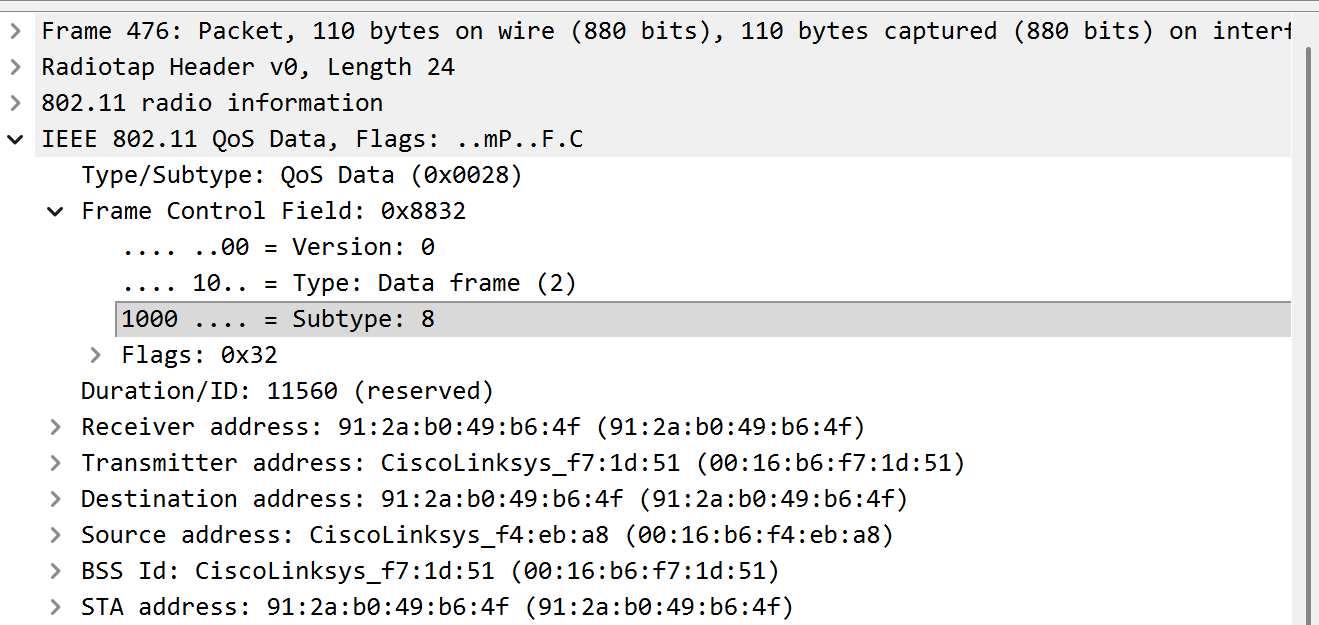
\includegraphics[width=0.95\linewidth]{graphics/fig8(1).png}
    \caption{Frame 476: 802.11 frame carrying the TCP SYNACK segment from the first-hop router to the wireless host.}
\end{figure}

% ==================== PHẦN 3: ASSOCIATION & DISASSOCIATION ====================
\newpage
\section{Association and Disassociation}

\subsection{Question 9}
\textbf{Question:} What two actions are taken (i.e., frames are sent) by the host in the trace just after t=49, to end the association with the 30 Munroe St AP that was initially in place when trace collection began? (Hint: one is an IP-layer action, and one is an 802.11-layer action). Looking at the 802.11 specification, is there another frame that you might have expected to see, but don’t see here?

\textbf{Answer:}
Right after $t=49\,\text{s}$, the host performs two distinct actions to terminate its session:
\begin{itemize}[noitemsep]
    \item \textbf{IP-layer action (Frame 1733, $t = 49.583615\,\text{s}$):} The host transmits a \textbf{DHCP Release} message to release its leased IP address (\texttt{192.168.1.109}) back to the DHCP server/gateway (\texttt{192.168.1.1}).
    \item \textbf{802.11-layer action (Frame 1735, $t = 49.609617\,\text{s}$):} The host sends an \textbf{802.11 Deauthentication frame} (\texttt{wlan.fc.subtype == 12}) directly to the \textit{30 Munroe St} AP (\texttt{00:16:b6:f7:1d:51}).
\end{itemize}
\textbf{Missing frame from 802.11 specification:} Under normal 802.11 procedures, a station ending an association is expected to send a \textbf{Disassociation frame} (\texttt{subtype 10}). However, in this trace, the station immediately sends a \textbf{Deauthentication frame} (\texttt{subtype 12}), which abruptly terminates both authentication and association in a single step without first disassociating.

\begin{figure}[H]
    \centering
    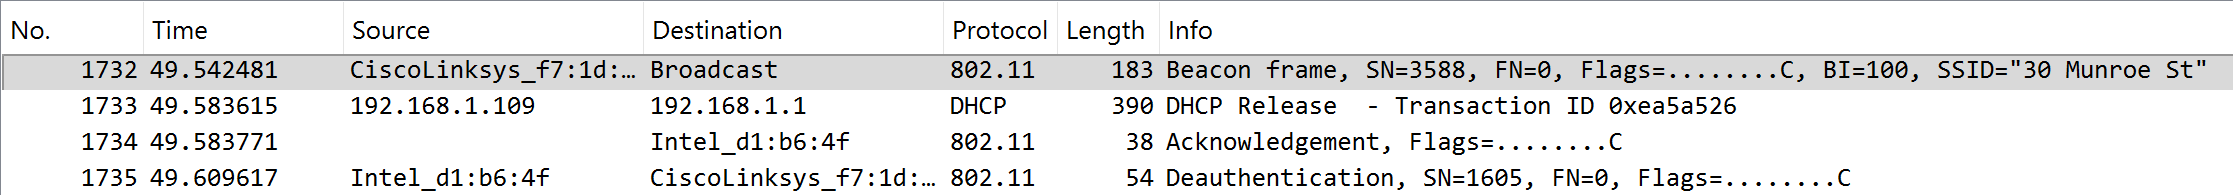
\includegraphics[width=0.98\linewidth]{graphics/fig9(1).png}
    \caption{Packet list showing Frame 1733 (DHCP Release at $t=49.58\,\text{s}$) and Frame 1735 (Deauthentication at $t=49.61\,\text{s}$).}
\end{figure}

\subsection{Question 10}
\textbf{Question:} Examine the trace file and look for AUTHENTICATION frames sent from the host to an AP and vice versa. How many AUTHENTICATION messages are sent from the wireless host to the linksys\_ses\_24086 AP (which has a MAC address of Cisco\_Li\_f5:ba:bb) starting at around t=49?

\textbf{Answer:}
Filtering by \texttt{wlan.fc.type\_subtype == 0x0b \&\& wlan.da == 00:18:39:f5:ba:bb}, we find that the host transmits exactly \textbf{6 AUTHENTICATION messages} to the \textit{linksys\_ses\_24086} AP:
\begin{itemize}[noitemsep]
    \item Frame 1740 ($t = 49.638857\,\text{s}$)
    \item Frame 1741 ($t = 49.639700\,\text{s}$)
    \item Frame 1742 ($t = 49.640702\,\text{s}$)
    \item Frame 1744 ($t = 49.642315\,\text{s}$)
    \item Frame 1746 ($t = 49.645319\,\text{s}$)
    \item Frame 1749 ($t = 49.649705\,\text{s}$)
\end{itemize}
The host sends an initial authentication request followed by 5 rapid retransmissions due to the lack of an authentication reply from the target AP.

\begin{figure}[H]
    \centering
    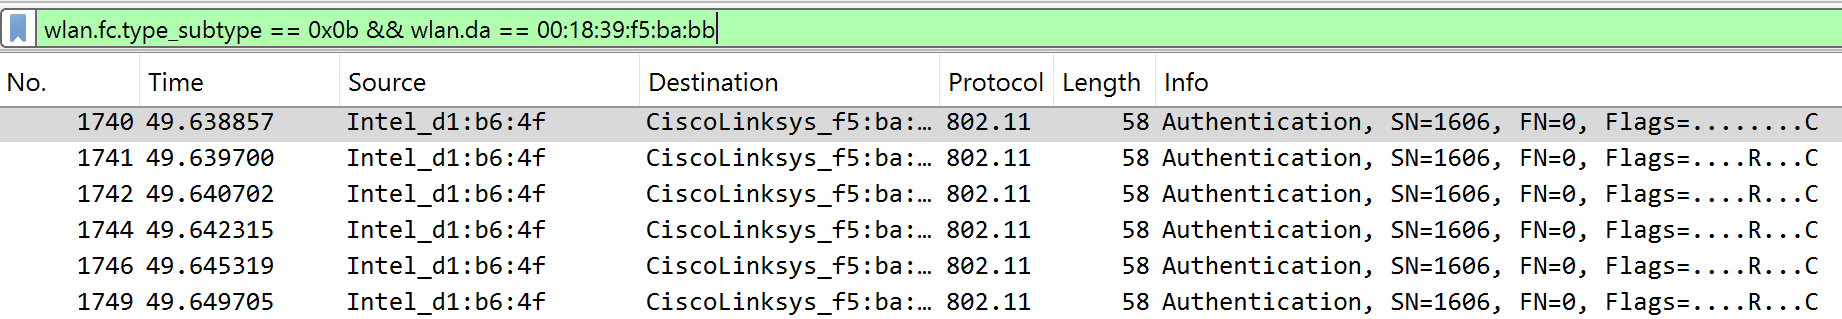
\includegraphics[width=0.98\linewidth]{graphics/fig10(1).png}
    \caption{Wireshark display showing the 6 Authentication frames sent by the host to \textit{linksys\_ses\_24086}.}
\end{figure}

\subsection{Question 11}
\textbf{Question:} Does the host want the authentication to require a key or be open?

\textbf{Answer:}
Looking at the Fixed Parameters field in Frame 1740:
\begin{itemize}[noitemsep]
    \item \textbf{Authentication Algorithm:} \textbf{Open System (0)}.
\end{itemize}
The host requests \textbf{Open System authentication}, meaning it does not require a shared key at the 802.11 link-layer authentication phase.

\begin{figure}[H]
    \centering
    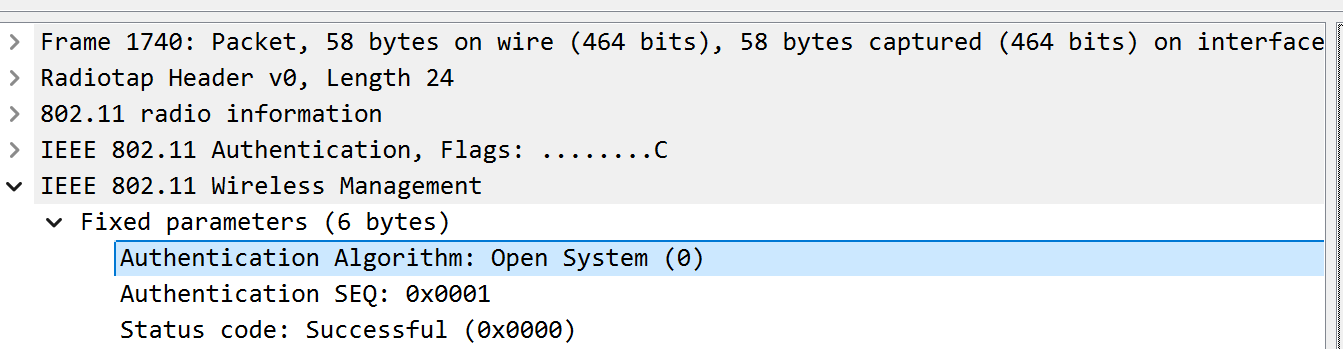
\includegraphics[width=0.95\linewidth]{graphics/fig11(1).png}
    \caption{Fixed parameters of Frame 1740 confirming \textit{Authentication Algorithm: Open System (0)}.}
\end{figure}

\subsection{Question 12}
\textbf{Question:} Do you see a reply AUTHENTICATION from the linksys\_ses\_24086 AP in the trace?

\textbf{Answer:}
\textbf{No.} Filtering for \texttt{wlan.fc.type\_subtype == 0x0b \&\& wlan.sa == 00:18:39:f5:ba:bb} returns \textbf{0 frames}. While the AP sends physical layer 802.11 ACK control frames, it never returns an 802.11 Management Authentication reply frame.

\begin{figure}[H]
    \centering
    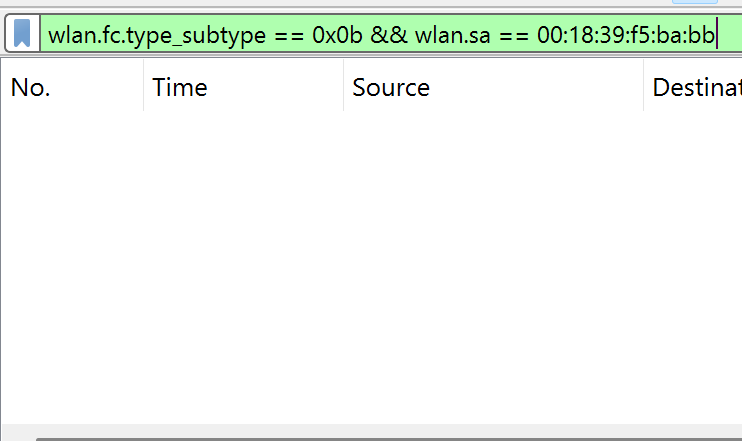
\includegraphics[width=0.95\linewidth]{graphics/fig12(1).png}
    \caption{Empty packet list confirming no reply Authentication frames were transmitted by \textit{linksys\_ses\_24086}.}
\end{figure}

\subsection{Question 13}
\textbf{Question:} Now let’s consider what happens as the host gives up trying to associate with the linksys\_ses\_24086 AP and now tries to associate with the 30 Munroe St AP. Look for AUTHENTICATION frames sent from the host to an AP and vice versa. At what times are there an AUTHENTICATION frame from the host to the 30 Munroe St. AP, and when is there a reply AUTHENTICATION sent from that AP to the host in reply?

\textbf{Answer:}
Using the filter \texttt{wlan.fc.subtype == 11 \&\& wlan.fc.type == 0 \&\& wlan.addr == 00:13:02:d1:b6:4f}:
\begin{itemize}[noitemsep]
    \item \textbf{Host $\rightarrow$ 30 Munroe St AP (Authentication Request):}
    \begin{itemize}[noitemsep]
        \item \textbf{Frame 2156} at \textbf{t = 63.168087 seconds} (Sequence number 1, Open System).
        \item \textbf{Frame 2160} at \textbf{t = 63.169707 seconds} (Retransmission).
    \end{itemize}
    \item \textbf{30 Munroe St AP $\rightarrow$ Host (Authentication Reply):}
    \begin{itemize}[noitemsep]
        \item \textbf{Frame 2158} at \textbf{t = 63.169071 seconds} (Status: Successful).
        \item \textbf{Frame 2164} at \textbf{t = 63.170692 seconds} (Status: Successful).
    \end{itemize}
\end{itemize}

\begin{figure}[H]
    \centering
    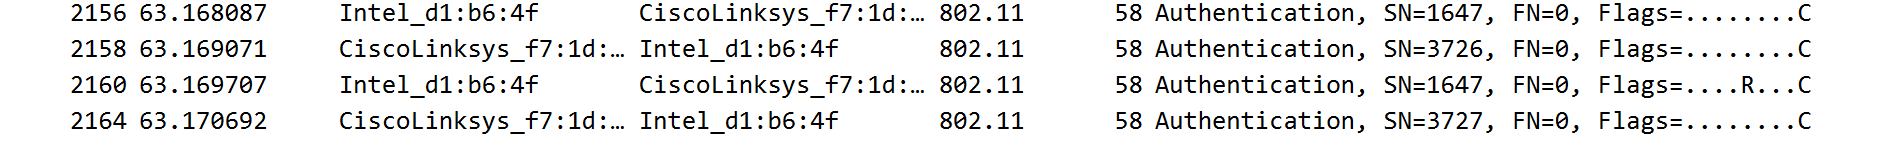
\includegraphics[width=0.98\linewidth]{graphics/fig13(1).png}
    \caption{Authentication exchange between the wireless host and \textit{30 Munroe St} around $t = 63\,\text{s}$ (Frames 2156, 2158, 2160, 2164).}
\end{figure}

\subsection{Question 14}
\textbf{Question:} An ASSOCIATE REQUEST from host to AP, and a corresponding ASSOCIATE RESPONSE frame from AP to host are used for the host to associate with an AP. At what time is there an ASSOCIATE REQUEST from host to the 30 Munroe St AP? When is the corresponding ASSOCIATE REPLY sent?

\textbf{Answer:}
Using the filter \texttt{wlan.fc.subtype < 2 \&\& wlan.fc.type == 0 \&\& wlan.addr == 00:13:02:d1:b6:4f}:
\begin{itemize}[noitemsep]
    \item \textbf{ASSOCIATE REQUEST (Host $\rightarrow$ AP):} \textbf{Frame 2162} at \textbf{t = 63.169910 seconds}.
    \item \textbf{ASSOCIATE RESPONSE (AP $\rightarrow$ Host):} \textbf{Frame 2166} at \textbf{t = 63.192101 seconds} (Status: Successful).
\end{itemize}

\begin{figure}[H]
    \centering
    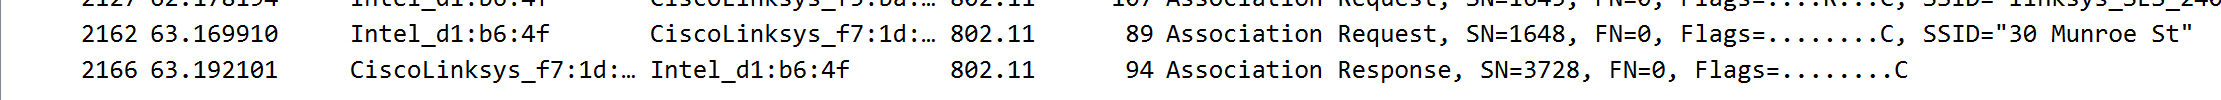
\includegraphics[width=0.98\linewidth]{graphics/fig14(1).png}
    \caption{Association Request (Frame 2162 at $63.17\,\text{s}$) and Association Response (Frame 2166 at $63.19\,\text{s}$).}
\end{figure}

\subsection{Question 15}
\textbf{Question:} What transmission rates is the host willing to use? The AP? To answer this question, you will need to look into the parameters fields of the 802.11 wireless LAN management frame.

\textbf{Answer:}
Examining the \textit{Tagged parameters} in the Association Request (\textbf{Frame 2162}) and Association Response (\textbf{Frame 2166}):
\begin{itemize}[noitemsep]
    \item \textbf{Host Transmission Rates (Frame 2162):}
    \begin{itemize}[noitemsep]
        \item \textit{Supported Rates (Tag 1):} 1.0, 2.0, 5.5, 11.0, 6.0, 9.0, 12.0, 18.0 Mbit/sec.
        \item \textit{Extended Supported Rates (Tag 50):} 24.0, 36.0, 48.0, 54.0 Mbit/sec.
        \item \textit{Combined Rates:} \textbf{1.0, 2.0, 5.5, 6.0, 9.0, 11.0, 12.0, 18.0, 24.0, 36.0, 48.0, 54.0 Mbit/sec}.
    \end{itemize}
    \item \textbf{AP Transmission Rates (Frame 2166):}
    \begin{itemize}[noitemsep]
        \item \textit{Supported Rates (Tag 1):} 1.0, 2.0, 5.5, 11.0 Mbit/sec.
        \item \textit{Extended Supported Rates (Tag 50):} 6.0, 9.0, 12.0, 18.0, 24.0, 36.0, 48.0, 54.0 Mbit/sec.
        \item \textit{Combined Rates:} \textbf{1.0, 2.0, 5.5, 6.0, 9.0, 11.0, 12.0, 18.0, 24.0, 36.0, 48.0, 54.0 Mbit/sec}.
    \end{itemize}
\end{itemize}
Both the host and the AP agree to support the exact same set of \textbf{12 data rates} (spanning 802.11b and 802.11g standards).

\begin{figure}[H]
    \centering
    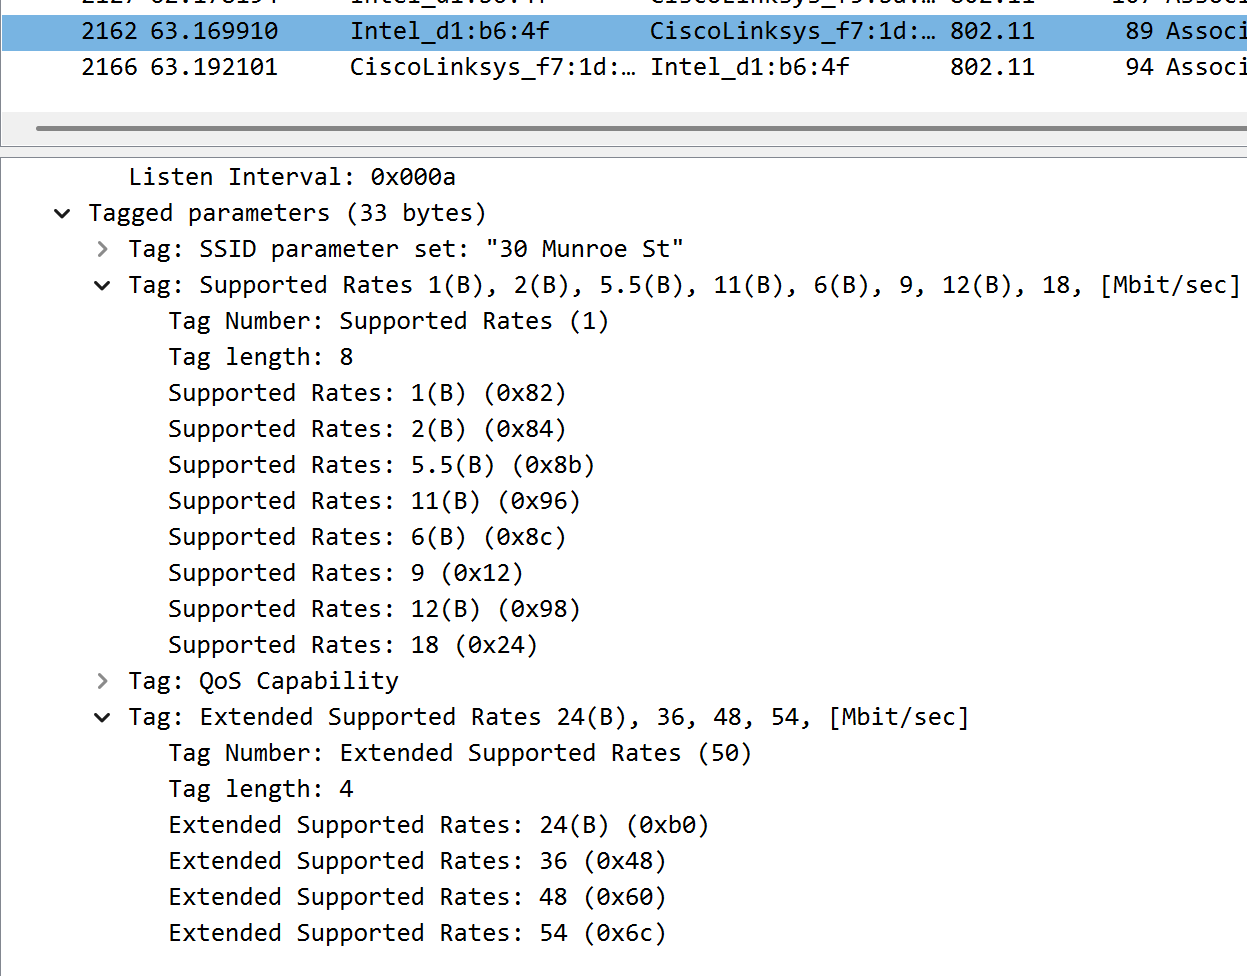
\includegraphics[width=0.95\linewidth]{graphics/fig15(1).png}
    \caption{Frame 2162: Transmission rates advertised by the host in Association Request.}
\end{figure}

\begin{figure}[H]
    \centering
    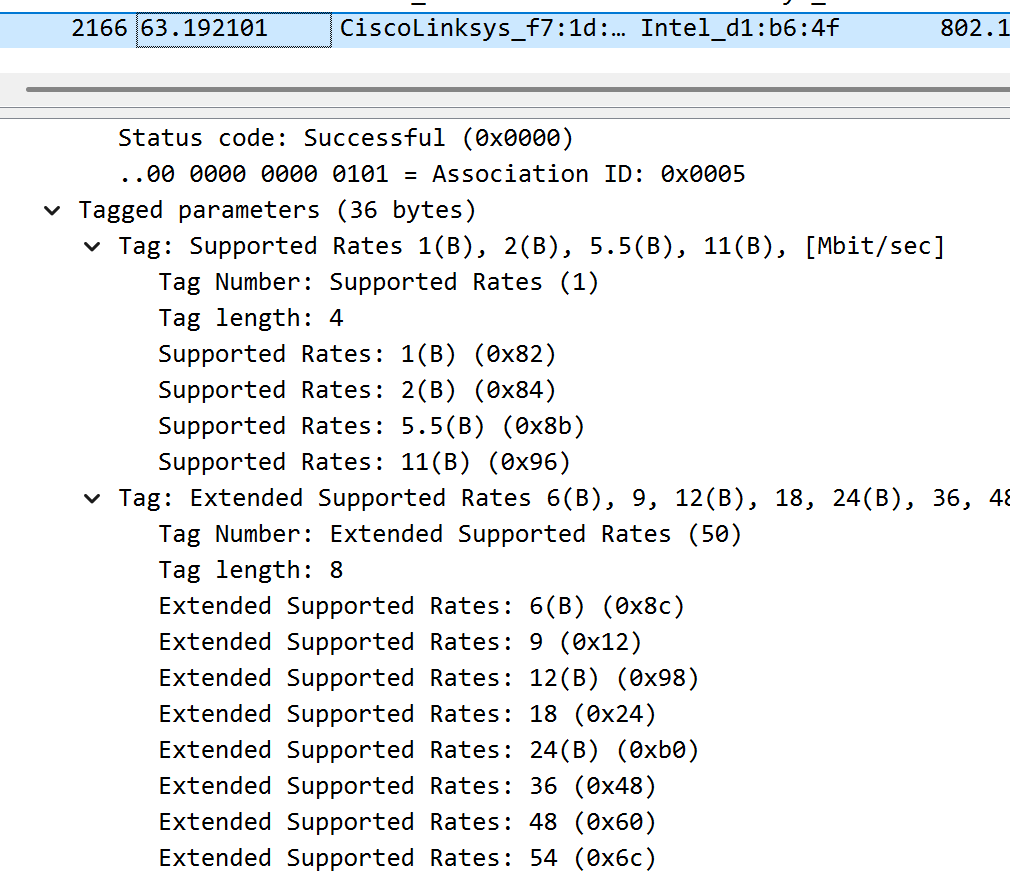
\includegraphics[width=0.95\linewidth]{graphics/fig15(2).png}
    \caption{Frame 2166: Transmission rates confirmed by the AP in Association Response.}
\end{figure}

% ==================== PHẦN 4: OTHER FRAME TYPES ====================
\newpage
\section{Other Frame Types}

\subsection{Question 16}
\textbf{Question:} Our trace contains a number of PROBE REQUEST and PROBE RESPONSE frames. What are the sender, receiver and BSS ID MAC addresses in these frames? What is the purpose of these two types of frames?

\textbf{Answer:}
\begin{enumerate}[label=\arabic*.]
    \item \textbf{Probe Request Frame (e.g., Frame 1737):}
    \begin{itemize}[noitemsep]
        \item \textbf{Receiver MAC (Address 1 / DA):} \texttt{ff:ff:ff:ff:ff:ff} (Broadcast).
        \item \textbf{Transmitter / Sender MAC (Address 2 / SA):} \texttt{00:13:02:d1:b6:4f} (\texttt{Intel\_d1:b6:4f}).
        \item \textbf{BSS ID (Address 3):} \texttt{ff:ff:ff:ff:ff:ff} (Wildcard BSSID).
        \item \textbf{Purpose:} Active network scanning. Wireless stations broadcast Probe Requests across radio channels to proactively discover available access points and query their parameters without passively waiting for beacon frames.
    \end{itemize}
    \item \textbf{Probe Response Frame (e.g., Frame 27):}
    \begin{itemize}[noitemsep]
        \item \textbf{Receiver MAC (Address 1 / DA):} \texttt{00:13:02:d1:b6:4f} (\texttt{Intel\_d1:b6:4f}).
        \item \textbf{Transmitter / Sender MAC (Address 2 / SA):} \texttt{00:16:b6:f7:1d:51} (\texttt{CiscoLinksys\_f7:1d:51}).
        \item \textbf{BSS ID (Address 3):} \texttt{00:16:b6:f7:1d:51} (\texttt{CiscoLinksys\_f7:1d:51}).
        \item \textbf{Purpose:} Sent by an AP as a unicast response to a Probe Request. It supplies the station with full network parameters (SSID, supported data rates, capability info) identical to a beacon, allowing the station to evaluate link quality and decide whether to associate.
    \end{itemize}
\end{enumerate}

\begin{figure}[H]
    \centering
    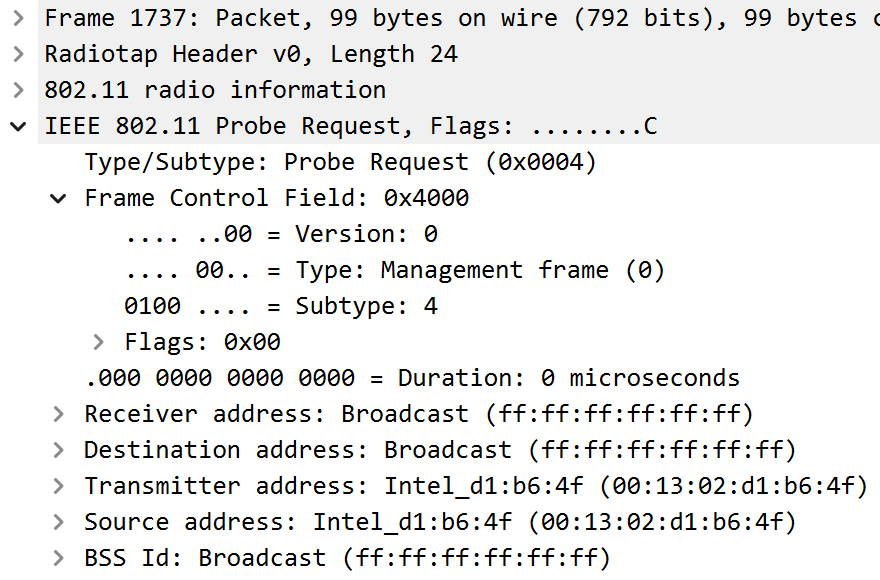
\includegraphics[width=0.95\linewidth]{graphics/fig16(1).png}
    \caption{Frame 1737: Probe Request broadcasted by the client to search for networks.}
\end{figure}

\begin{figure}[H]
    \centering
    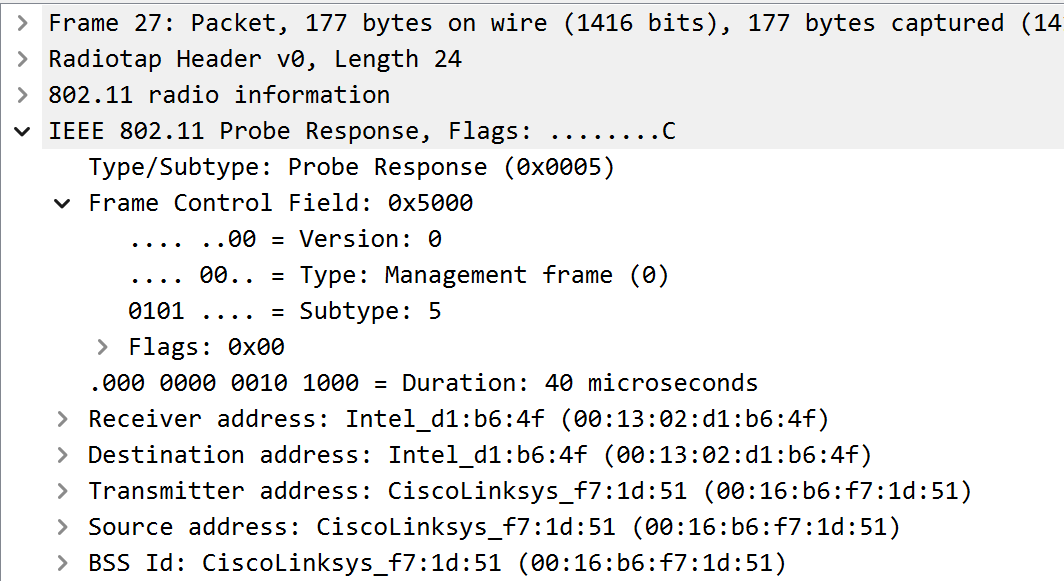
\includegraphics[width=0.95\linewidth]{graphics/fig16(2).png}
    \caption{Frame 27: Probe Response sent by the AP directly to the client.}
\end{figure}

\end{document}
